\documentclass[11pt]{article}
\usepackage{acl2014}
\usepackage{times}
\usepackage{url}
\usepackage{latexsym}
\usepackage{graphicx}
\usepackage{adjustbox}
\usepackage{array}
\usepackage{booktabs}
\usepackage{multirow}
\usepackage{multicol}% http://ctan.org/pkg/multicols
\usepackage{tabularx, booktabs}
\usepackage{framed}
\usepackage{setspace} 

% Change this if needed to set titlebox size.
%\setlength\titlebox{5cm}

\title{LING 573: Final Project Report}

\author{Clara Gordon \\
  University of Washington \\
  Seattle, WA \\
  {\tt cgordon1@uw.edu} \\\And
  Claire Jaja \\
  University of Washington \\
  Seattle, WA \\
  {\tt cjaja@uw.edu} \\\And
  Andrea Kahn \\
  University of Washington \\
  Seattle, WA \\
  {\tt amkahn@uw.edu} \\}

\date{}

\begin{document}
\maketitle
\begin{abstract}

In this paper, we describe a question answering system for handling factoid questions.  The system, implemented in Python, follows a typical pipeline, including query processing, information retrieval, and answer candidate extraction and ranking modules. Using the AQUAINT corpus of English News Text as a document collection, it produces answers for questions from the QA track of the Text Retrieval Conference (TREC).

\end{abstract}

\section{Introduction}

Question answering (QA) has long been a prominent problem in the field of natural language processing. In contrast to information retrieval (IR) systems, which return relevant documents based on search terms, a question answering system takes a natural-language question as input and outputs a natural-language answer. IR is typically a component of the system, but the addition of question and answer processing prevents users from having to sift through long documents to find the information they are seeking.

We implemented a question answering system, the Question Answering Integrated Linguistic System (QuAILS) (see logo in Figure 1), to handle factoid questions from the QA track of the Text Retrieval Conference (TREC), using the AQUAINT Corpus of English News Text as a document collection.  Our system achieves lenient MRR scores in the upper .30s, meaning that, on average, the correct answer appears third in the list of answers returned.

\begin{figure}
\centering

\includegraphics[width=0.5\textwidth]{QuAILS.jpg}
\caption{QuAILS logo.}
\end{figure}

\section{System Overview}

Our system is coded in Python. Third-party modules that we use include Indri/Lemur (for IR), pymur (a Python wrapper for Indri/Lemur), Beautiful Soup (for XML parsing), and NLTK (for tokenization, part of speech tagging, named entity chunking, and thesaurus-based query expansion). We chose Indri/Lemur for IR because of its specific handling of TREC-formatted question files. We use a stopword list taken from the Indri/Lemur documentation.

We use Indri's IndriBuildIndex code to build an index.  It has a parameter file specified as an argument which gives the path to the document collection, the path to the output index, and other parameters.  Indexing of the AQUAINT corpus takes approximately 15 minutes.  We created several different versions of the index, using both Porter and Krovetz stemmers, both including and excluding a list of stopwords. Having found previous best results with the Porter-stemmed index including a stopword list, we conducted our final set of tests using that particular index and opted to construct the index for the AQUAINT-2 corpus with those parameters as well.

The core of our system is a three-part pipeline, consisting of modules for question processing, IR, and answer processing, respectively. The system architecture is shown in Figure 2.

\begin{figure}
  \centering
    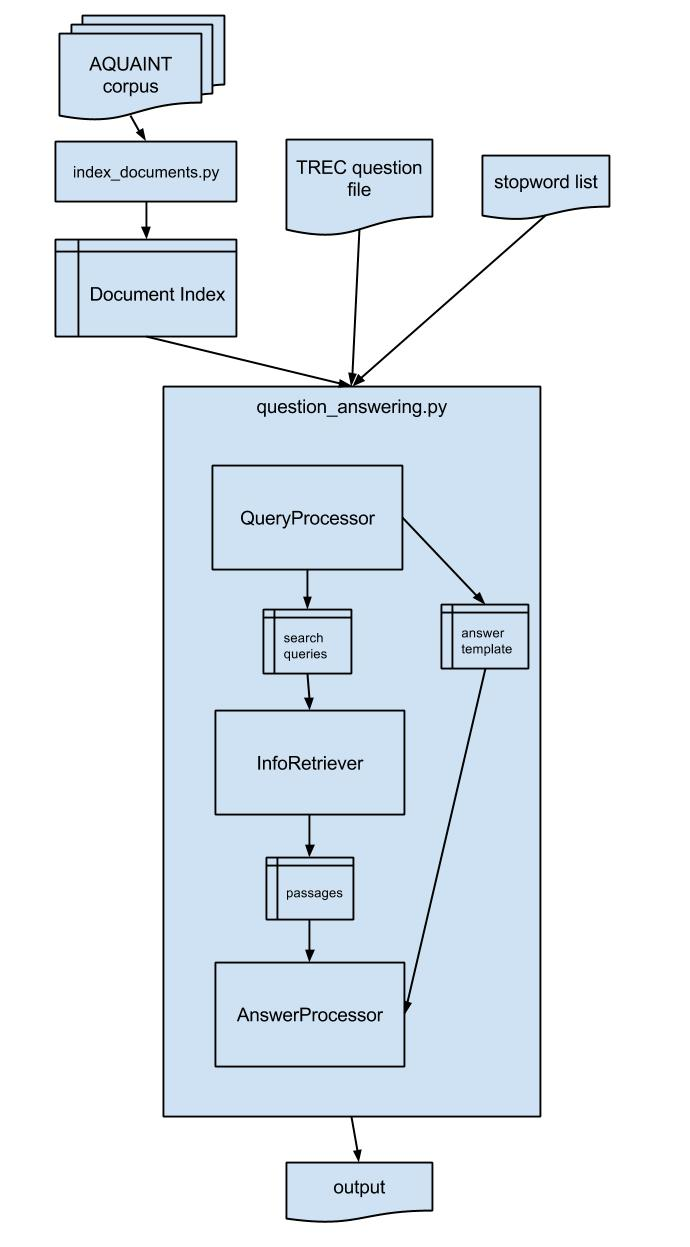
\includegraphics[width=0.5\textwidth]{system_architecture.jpg}
 \caption{System architecture.}
\end{figure}

\section{Approach}

The question answering system is called by a wrapper script, question\_answering.py, which take a mandatory run tag argument and 20 optional system parameters (see Table 1). It uses the third-party module Beautiful Soup to parse the XML in the TREC document and generate a list of questions. Python's multiprocessing module is used to parallelize the questions in the question file, so that multiple questions may be passed through the pipeline (described in detail below) at once. For each in the group of answers returned for each question, the wrapper script prints the question ID, the run tag, the document ID associated with the answer, and the answer to the output file.

A separate script, cache\_web\_results.py, submits each unprocessed factoid query to Ask.com for later use in query expansion and information retrieval. We omit any query processing in this portion of the system because we assume Ask.com has its own query processing algorithms which can better handle the raw query. The script uses BeautifulSoup to scrape the text snippets associated with each result, and stores them in a text document in the cached\_web\_results directory. After running several experiments, we have found that four pages of results is optimal.

\begin{table*}[!ht]
  \centering
  \caption{Parameters (Note: Settings displayed are those used for the final evaluation run.)}
  \renewcommand{\arraystretch}{1.5}% Spread rows out...
    \begin{tabular}{>{\centering\bfseries}m{.5in} >{\centering}m{2in} >{\centering}m{2in} >{\centering\arraybackslash}m{1in} }
    \toprule
\textbf{Category} & \textbf{Parameter} & \textbf{Description} & \textbf{Setting} \\
    \midrule
General & q\_file & filepath of TREC question file & /dropbox/13-14/573/Data/Questions/evaltest/ QA2007\_testset.xml \\
& stoplist & filepath of list of stopwords & src/stoplist.dft \\
& web\_cache & filepath of cached Ask.com web results & src/cached\_web\_results/ QA2007\_testset. 4pg.web\_cache \\
& index & filepath of Indri index &  src/indexes/AQUAINT-2/porter.stoplist  \\
QP & stopword\_filter\_target  &  whether to perform target stopword filtering & False \\
& target\_upweighting & upweighting factor for target terms &  1 \\
& ne\_upweighting & upweighting factor for NEs & 1 \\
& num\_web\_exp\_terms  &   number of web-redundancy terms added to query & 5 \\
& weight\_web\_exp\_terms  & weight of web-redundancy terms & 0.5  \\
& num\_lin\_exp\_terms & number of Lin-thesaurus terms added to query & 0  \\
& weight\_lin\_exp\_query & weight given to Lin-thesaurus-expanded query & 0 \\
IR & indri\_passages & number of passages returned Indri & 20 \\
& passage\_length & character length of passage returned by indri & 75 \\
& indri\_window\_size  &  size of window in Indri search & 30 \\
& snippet\_weight & weight assigned to web snippets & 0.9 \\
AP & num\_docs & number of AQUAINT docs answer must occur in & 1 \\
& num\_passages & number of passages answer must occur in &  10 \\
& snippet\_passage\_count &  how many passages a web snippet counts as  & 10 \\
& passages\_per\_doc\_id & number of passages to return per document ID & 1  \\
    \bottomrule
  \end{tabular}
\end{table*}


%\begin{table*} 
%    \begin{center}
%      \resizebox{\linewidth}{!}{
%\begin{tabular}{|l|l|l|l|}
%\hline
%\textbf{Category} & \textbf{Parameter} & \textbf{Description} & \textbf{Setting} \\ \hline
%General & q\_file & filepath of TREC question file & /dropbox/13-14/573/Data/Questions/evaltest/QA2007\_testset.xml %\\\cline{2-4}
%& stoplist & filepath of list of stopwords & src/stoplist.dft \\\cline{2-4}
%& web\_cache & filepath of cached web Ask.com web results & src/cached\_web\_results/QA2007\_testset.4pg.web\_cache %\\\cline{2-4}  
%& index & filepath of Indri index &  src/indexes/AQUAINT-2/porter.stoplist  \\\hline
%QP & stopword\_filter\_target  &  whether to perform target stopword filtering & False \\\cline{2-4}
%& target\_upweighting & \pbox{20cm} upweighting factor for target terms &  1   \\\cline{2-4}
%& ne\_upweighting & \pbox{20cm} upweighting factor for NEs & 1 \\\cline{2-4}
%& num\_web\_exp\_terms  &   number of web-redundancy terms added to query & 5 \\\cline{2-4}
%& weight\_web\_exp\_terms  & weight of web-redundancy terms & 0.5  \\\cline{2-4}
%& num\_lin\_exp\_terms & number of Lin-thesaurus terms added to query & 0  \\\cline{2-4}
%& weight\_lin\_exp\_query & weight given to Lin-thesaurus-expanded query & 0 \\\hline
%IR & indri\_passages & number of passages returned Indri & 20 \\\cline{2-4}
%& passage\_length & character length of passage returned by indri & 75 \\\cline{2-4}  
%& indri\_window\_size  &  size of window in Indri search & 30 \\\cline{2-4}
%& snippet\_weight & weight assigned to web snippets & 0.9 \\\hline
%AP & num\_docs & number of AQUAINT docs answer must occur in & 1 \\\cline{2-4}
%& num\_passages & number of passages answer must occur in &  10 \\\cline{2-4}
%& snippet\_passage\_count &  how many passages a web snippet counts as  & 10 \\\cline{2-4}
%& passages\_per\_doc\_id & number of passages to return per document ID & 1  \\\cline{2-4} 
%& passages\_per\_answer\_candidate & number of passages to return per answer candidate & 1  \\ \hline
%\end{tabular}}
%\vspace{1mm}
%\emph{Table xxx: Parameters (Note: Settings displayed are those used for the final evaluation run.)}
%\end{center}
%\end{table*}


Classes that are used by multiple modules in the pipeline are defined in the module general\_classes.py. These include:

\begin{itemize}
\item Question class: A Question object stores as attributes the TREC question ID, the question type, the TREC natural-language question stored as a string, and the ``target" (the context given for a set of questions in TREC 2004-2006; defaults to None).
\item SearchQuery class: A SearchQuery object stores as attributes a dictionary of search terms, each of which can be one or more words, mapped to weights indicating how important those terms are perceived as being, and an overall weight for the query, which will be used to calculate the probability of the corresponding AnswerCandidate.
\item AnswerTemplate class: An AnswerTemplate object stores as attributes the question ID, a set of basic search query terms from the original question, and a dictionary for the weights of each answer type, where the weights will be used to reweight AnswerCandidate objects during answer processing.
\item Passage class: A Passage object stores as attributes the text of a snippet, its weight, and the document ID.
\end{itemize}

\subsection{System architecture}

Our pipeline for processing a single question consists of three components found in three separate modules, described below. The pipeline takes a Question object as input and outputs a list of AnswerCandidate objects.

\subsubsection{Query processing}

The query processing module is responsible for creating a set of weighted search queries (which are passed to the information retrieval module to be used for passage retrieval) and instantiating an answer template (which is passed to the answer processing module to be used during answer ranking).

A QueryProcessor object is initialized with a Question object, a stopword list, and a set of cached web snippets. It then generates a vocabulary, or a list of words (i.e., whitespace-tokenized strings) occurring in the question/target and their counts. We use NLTK's named-entity chunker to remove named entities from the question before tokenizing to prevent the named entities themselves from being tokenized. (Performing named entity chunking on the target caused our accuracy to drop significantly, so we chose to forgo named entity chunking of the target and did not consider target tokens when performing Lin thesaurus-based query expansion.) The named entities are then added back into the set of query terms when the queries are generated. We experimented with upweighting the named entities, but our final set of parameter values did not include named entity upweighting (i.e., the ne\_upweighting parameter was set to its default value of 1). Some implementation decisions made during this step drastically affected our scores; in addition to performing or not performing named entity chunking on the target, the choice as to whether or not to filter stopwords from the target also had a significant effect on our score. (We made stopword\_filter\_target a boolean parameter with the default value of False, and found this setting to be optimal.)

After instantiating a QueryProcessor object, the wrapper script then calls a method in the query-processing module that instantiates an AnswerTemplate object that will subsequently be passed to the answer processing module. The answer template contains the query processor's vocabulary so that the answer processing module can disregard answer candidates that contain query terms. In addition, this method employs regular-expression matching on the original natural-language question to identify questions as requiring an answer that is the name of a person (i.e., proper noun), the name of an organization (i.e., proper noun), the name of an object (i.e., common noun), the name of a location (i.e., proper noun), a time expression, a number expression, or some expression that does not fall into one of these categories. Some regular expressions correspond to one of these answer types; others correspond to multiple answer types. A regular expression match causes the corresponding answer types to be given a higher weight in the AnswerTemplate dictionary of answer type weights. In the final version of the system, we set the weights of answer types matched by a regular expression to 0.9, the weights of all other answer types to 0.1, and the weight of ``other" to 0.5 if no regular expression matches. (These are weights, not probabilities, so the choice of scale is somewhat arbitrary; what matters is their magnitude relative to one another.)

The query processor is then used to generate a list of weighted search queries, each of which is in turn a set of weighted search terms. In the final version of the system, the query processor generates three queries: an initial search query that contains the set of words occurring in the question and the question target, with the word counts as weights and the query weight set to 1; a web-expanded version of the initial query, with the weights of the expanded terms taken as a parameter and the query weight set to 1; and a Lin thesaurus-expanded version of the initial query, with the weights of the expanded terms set by the Lin expansion function (see below) and the query weight taken as a parameter.

We implemented two types of query expansion: web-based and Lin thesaurus-based. Web-based query expansion adds the \emph{n} most frequently appearing unigrams in the web snippets associated with a question (not including stopwords or words already appearing in the query) to the original set of weighted query terms, assigning these terms some default weight. An n value and a weight for the terms are passed to the query processing module as parameters, with default values 5 and 0.5, respectively; we found these parameters to be optimal given the combinations we tested (though with more time, we would have chosen to test these parameters more extensively; see Discussion).

We also implemented query expansion using NLTK's thesaurus corpus from \newcite{lin1998automatic} and its associated scored\_synonyms method, which returns similar terms grouped by part of speech (noun, verb, or adjective). Our expand\_query method returns a SearchQuery object containing all of the original query terms and their corresponding weights, as well as the top \emph{n} synonyms for certain query terms, their weights being the product of the weight of the original term of which they are synonyms and the weight returned by scored\_synonyms. To determine which query terms to expand, we performed part of speech-tagging on the original question text, followed by named entity-chunking (both using NLTK), and only expanded non-named entity terms that did not appear in the stopword list; in addition, we only expanded terms that were tagged as nouns or verbs and only returned related thesaurus terms classified by the thesaurus as being nouns or verbs, respectively. An \emph{n} value and a weight for this expanded query are passed as parameters, with default values of 0 and 0. We tested several non-default values of these parameters and found that changing these values negatively affected our MRR, so we did not make use of Lin query expansion in our final run.

\subsubsection{Information retrieval}

The information retrieval module uses the Indri/Lemur IR system to retrieve \emph{n} passages for each set of query terms passed to it by the query processing module, where \emph{n} is a parameter. Empirical tests show that returning 20 Indri passages provides the best results. We use Base64 conversion for our queries in order to avoid encoding errors with punctuation. Although we use Indri directly to index the document collection, this portion of the system uses the pymur wrapper to run the query and retrieve passage results. We use the given offset indices to retrieve the passage from the original text. Since these indices refer to the stemmed text, however, the passages may be a slightly different window from that selected by Indri. The pymur commands provide the document ID number and document weight. Together with the reconstructed passage text, these are used to construct a Passage object for each passage. 

We make use of certain Indri Query Language functionalities in addition to Base64 conversion. Because some of the ``tokens" contained in the Query objects are in fact space-delimited named entity phrases, the syntax of the Indri query treats each token as ordered window that must be matched completely. Each of these windows are weighted according to the weights specified in the Query object. The length of the returned passage and search window are also specified by parameters. We found the best results using passages of a length of 75 words and a search window of length 30. 

We implement web boosting by using the cached web results stored before runtime to augment the returned passages. These cached results are retrieved and stored as Passage objects, similar to the AQUAINT passages. The weights of these passages are also parameterized in our script. Initial experiments showed that these web snippets are very likely to contain the answer, and we weight them similarly to a very high scoring AQUAINT document in our IR framework: log(0.9).  The document ID for these Passage objects is set to None to indicate that these are web snippets, not passages coming from AQUAINT documents.  Together, the AQUAINT and web-based Passage objects are passed on to the answer extraction module. 


\subsubsection{Answer candidate extraction and ranking}

The answer processing module is used to extract and rank answers.  An object of this class is initialized with a list of Passage objects, an AnswerTemplate object, and an optional stopword list.  This object can then generate and rank answers.  This is done in a series of steps, inspired by \newcite{lin2007exploration}.

First, possible answers are extracted from the Passages by generating all unigrams, bigrams, trigrams, and 4-grams from the text of each passage; the score of each of these possible answers is the sum of the retrieval scores of the passage it is found in.  If an n-gram appears multiple times in a passage, the n-gram's score is updated each time the n-gram appears, so a possible answer that appears frequently in a passage is scored higher than one that appears just once in the passage. At the end, a list of AnswerCandidate objects is generated which contains the question ID, a possible answer, its score, the document collection documents (and specific passages within those documents) it is found in, and the total number of passages it is found in.  Since we believe that the web snippets are more likely to contain the correct answer than the documents from the document collection, we allow each web snippet to count as \emph{n} passages, where \emph{n} is a parameter passed in to the wrapper script, with a default value of 10.  We found best results with this default value.

After this, the answer candidates go through a filtering step.  At this step, any answers that start or end with a stopword or standalone punctuation token, or contain any words from the original query (retrieved from the AnswerTemplate) are discarded.  Additionally, any answers that did not appear in at least \emph{m} document collection documents are discarded, and any answers that did not appear in at least \emph{p} total passages are discarded, where \emph{m} and \emph{p} are parameters passed in to the wrapper script, with default values of \emph{m} = 1 and \emph{p} = 10.  We found best results with these default values.

Then, a combining step updates the score of each answer to be the current score plus the sum of the scores of the unigram answers contained within it. This prevents unigrams from being the highest ranked answers and instead favors longer answers.

Next, the answers are reweighted.  Regular expressions are used to guess the type of each answer.  Three different categories are captured; 1) person, organization, or location (identified by an answer beginning with a capital letter), 2) time expression (identified by an answer containing month words or a pattern resembling a date), and 3) numbers (identified by digits as well as number words).  Then, the weights from the AnswerTemplate are applied accordingly.  Since person, organization, and location are not distinguished in the answers, the highest weight among these three in the AnswerTemplate is used for any answer identified as being in that category.

Then, the answer candidates are ranked by score.  AQUAINT passages are chosen based on these n-gram answers, given a few different criteria.  Up to \emph{q} passages are returned per answer candidate, with up to \emph{r} passages per document ID for allowed for the question.  These parameters are set by default to \emph{q} = 1 and \emph{r} = 1, and these default values gave the best results in our tests.  Starting at the highest-ranked answer candidate, the document ID which contributed the most passages containing that answer candidate is returned, along with the passage from that document ID with the highest Indri retrieval score, provided that the maximum number of passages per document ID (parameter \emph{r}) for that document ID has not already been met.  The passage is truncated to 250 characters, centered on the occurrence of the n-gram answer candidate.  This continues (moving on to the document ID which contributed the next most passages) until the maximum number of passages per answer candidate (parameter \emph{q}) has been reached for that answer candidate, and then the process continues with the next highest ranked answer candidate.

\section{Results}

We evaluated our results using the mean reciprocal rank (MRR) measure with strict and lenient evaluation.  The results, based on automatic pattern scoring, are shown in the tables below.  All scores are rounded to four significant digits.

\begin{table}[ht]
  \centering
  \caption{Passage retrieval experiments on dev-test data.}
  \renewcommand{\arraystretch}{1.5}% Spread rows out...
    \begin{tabular}{>{\centering\bfseries}m{.5in} >{\centering}m{1in} >{\centering\arraybackslash}m{1in} }
    \toprule
\textbf{Passage Count} & \textbf{Strict Score} & \textbf{Lenient Score} \\
    \midrule
20 & 0.2072	& 0.3580 \\
40 & 0.1922 & 0.3514 \\
60 & 0.1837	& 0.3380 \\
80 & 0.1667	& 0.3282 \\
    \bottomrule
  \end{tabular}
\end{table}


\begin{table}[ht]
  \centering
  \caption{Web cache experiments on dev-test data.}
  \renewcommand{\arraystretch}{1.5}% Spread rows out...
    \begin{tabular}{>{\centering\bfseries}m{.5in} >{\centering}m{1in} >{\centering\arraybackslash}m{1in} }
    \toprule
\textbf{Webpage Count} & \textbf{Strict Score} & \textbf{Lenient Score} \\
    \midrule
2 & 0.1871 & 0.3480 \\
3 & 0.1922 & 0.3514 \\
4 & 0.1913 & 0.3524 \\
    \bottomrule
  \end{tabular}
\end{table}

\begin{table}[ht]
  \centering
  \caption{Indri search experiments on dev-test data.}
  \renewcommand{\arraystretch}{1.5}% Spread rows out...
    \begin{tabular}{>{\centering\bfseries}m{.5in} >{\centering\bfseries}m{.5in} >{\centering}m{.75in} >{\centering\arraybackslash}m{.75in} }
    \toprule
\textbf{Passage Length} & \textbf{Window Length} & \textbf{Strict Score} & \textbf{Lenient Score} \\
    \midrule
75 & 30 & 0.1979 & 0.3680 \\
100 & 50 & 0.1922 & 0.3514 \\
150	& 75 & 0.1835	& 0.3394 \\
    \bottomrule
  \end{tabular}
\end{table}

\begin{table}[ht]
  \centering
  \caption{Final results}
  \renewcommand{\arraystretch}{1.5}% Spread rows out...
    \begin{tabular}{>{\centering\bfseries}m{.75in} >{\centering}m{.75in} >{\centering\arraybackslash}m{.75in} }
    \toprule
\textbf{Deliverable} & \textbf{Strict Score} & \textbf{Lenient Score} \\
    \midrule
D2 & 0.0051 & 0.0289 \\
D3 & 0.1451 & 0.2639 \\
D4 (dev) & 0.2160 & 0.3773 \\
D4 (eval) & 0.1766 & 0.3584 \\
    \bottomrule
  \end{tabular}
\end{table}

\section{Discussion}

One of the salient takeaways of this project was that shallow and redundancy-based techniques go a long way. We achieved lenient MRR scores in the high .30s without doing any sort of deep processing (e.g., parsing, query reformulation, minimal recursion semantics), with especially large gains from web-based query expansion and the use of web snippets in generating and ranking answer candidates. With more time, we believe we could have attained even higher MRR scores through augmenting our system to employ some of the aforementioned deep processing techniques.

In terms of implementation, the choice to parallelize the processing of each question and the choice to pass as parameters to our wrapper script were immensely helpful. Our final system ran in approximately five minutes with a single job on our shared computing cluster. We were able to run 55 experiments on the development data and chose the set of parameter values that gave the highest MRR scores as the parameter settings for our final evaluation test run.

A limiting factor in determining optimal parameter settings was computing power. We believe that we would have been able to achieve higher scores had we been able to run more experiments. We chose combinations of parameters to test largely by isolating one parameter and varying it across several experiments while keeping other parameters consistent. Unfortunately, this doesn't capture how the parameters interact with one another, and we have reason to believe that many of them do (e.g., number of pages of web-cached results and number of web-based expansion terms). However, even assuming an average of three desired test settings for each parameter, testing every combination of values for 20 parameters would mean running $3^{20}$ (approximately 3.5 billion) experiments. Needless to say, this was not realistic given our computing cluster and the project timeline.

The results of the experiments we ran showed the biggest improvements with tweaks to parameters within information retrieval and in regards to web results.  In particular, returning fewer document collection passages within Indri gave us better results (see Table 2).  Additionally, we experimented with the passage and window length for our Indri queries, with results showing that a passage of 75 words with a 30 word window gave the best results (see Table 3).  In terms of web results, we tested varying the number of pages of web search results for our cached web snippets; the best results were with three pages (for strict results) and four pages (for lenient results) (see Table 4).  For brevity, details are not included on our other experiments.  The results with the final best settings for the parameters (see Table 1 for a full list of what these settings are) are shown in the last two rows of Table 5.  These results show a significant improvement over our results for previous deliverables (shown in the first two rows of the table) and illustrate a consistent improvement of our overall system throughout the past ten weeks.

Error analysis (see Table 6) on our final results show that we return the correct answer in our 20 responses 58.6\% of the time for the development set and 57.2\% of the time for the evaluation set.  About half of these correct answers are returned as the first answer.  A much larger number, however, are returned within the top 3.  If we were able to improve our ranking so that when the correct answer is in the top three, it is the first one, we would have had lenient scores over .451 for the development set and .428 for the evaluation set.  This doesn't include correct answers that we returned further down in the list.  Thus, it seems like reranking would be a fruitful endeavor for improving the MRR scores.

However, additionally, this means that nearly half the questions do not have a correct answer anywhere in the answers returned.  Improvements to answer generation and passage return may thus also be a possible arena for improving the scores.

%\begin{center}
%\begin{tabular}{|*{3}{c|}}
%\hline
% & \textbf{2006 (dev test)} & \textbf{2007 (eval test)} \\ \hline
%{\parbox[t][10mm]{30mm}{\center{\# of questions w/ answer patterns}}} & 386 & 290 \\ \hline
%{\parbox[t][10mm]{30mm}{\center{\# of questions where QuAILS returned correct answer}}} & 226 & 166 \\ \hline
%{\parbox[t][20mm]{30mm}{\center{\# of questions where QuAILS returned correct answer in top 10}}} & 224 & 161 \\ %\hline
%{\parbox[t][20mm]{30mm}{\center{\# of questions where QuAILS returned correct answer in top 3}}} & 174 & 124 \\ %\hline
%{\parbox[t][20mm]{30mm}{\center{\# of questions where QuAILS returned correct answer as first answer}}} & 107 & 73 %\\ \hline
%\end{tabular}
%\vspace{1mm}
%\emph{Table xxx: Error Analysis.}
%\end{center}

\begin{table}[ht]
  \centering
  \caption{Error Analysis}
  \renewcommand{\arraystretch}{1.5}% Spread rows out...
  \begin{tabular}{>{\centering\bfseries}m{1.2in} >{\centering}m{.5in} >{\centering\arraybackslash}m{.5in} }
    \toprule
     & \textbf{2006 (dev)} & \textbf{2007 (eval)} \\
    \midrule
    \# of questions w/ answer patterns & 386 & 290 \\
    \# of questions where QuAILS returned correct answer & 226 & 166 \\
    \# of questions where QuAILS returned correct answer in top 10 & 224 & 161 \\
    \# of questions where QuAILS returned correct answer in top 3 & 174 & 124 \\
    \# of questions where QuAILS returned correct answer as first answer & 107 & 73 \\
    \bottomrule
  \end{tabular}
\end{table}


\section{Conclusion}

We implemented a question answering system to handle factoid questions from the TREC QA shared task using the AQUAINT Corpus as a document collection.  We experimented with question classification, query expansion using web cached snippets, and Lin synonym-based query expansion.  Within information retrieval, we tested using different Indri parameters, as well as including web cached snippets as passages.  For answer processing, we implemented ARANEA-style n-gram generation, filtering, and ranking.  Through these various experiments, we were able to achieve lenient MRR results on both the development and test sets in the upper .30s and strict MRR results around .20.

\nocite{*}
\bibliographystyle{acl}
\bibliography{references}

%\begin{thebibliography}{}

%\end{thebibliography}

\end{document}


